\documentclass[twoside,11pt]{article}

% ? Specify used packages
\usepackage{graphicx}        %  Use this one for final production.
% \usepackage[draft]{graphicx} %  Use this one for drafting.
% ? End of specify used packages

\pagestyle{myheadings}

% -----------------------------------------------------------------------------
% ? Document identification
% Fixed part
\newcommand{\stardoccategory}  {Starlink User Note}
\newcommand{\stardocinitials}  {SUN}
\newcommand{\stardocsource}    {sun\stardocnumber}

% Variable part - replace [xxx] as appropriate.
\newcommand{\stardocnumber}    {45.16}
\newcommand{\stardocauthors}   {Nicholas Eaton, Peter W.\ Draper \& Alasdair Allan}
\newcommand{\stardocdate}      {27th November 2009}
\newcommand{\stardoctitle}     {PHOTOM --- A Photometry Package }
\newcommand{\stardocversion}   {Version 1.12-0}
\newcommand{\stardocmanual}    {User's Manual}
\newcommand{\stardocabstract}  {
  \begin{center}
    \htmlref{PHOTOM}{PHOTOM} is a package for measuring the sky corrected
    magnitudes and fluxes of astronomical objects, within circular and
    elliptical apertures, using either the aperture or optimal extraction
    algorithms.
  \end{center}
  }
% ? End of document identification
% -----------------------------------------------------------------------------

% +
%  Name:
%     sun.tex
%
%  Purpose:
%     Template for Starlink User Note (SUN) documents.
%     Refer to SUN/199
%
%  Authors:
%     AJC: A.J.Chipperfield (Starlink, RAL)
%     BLY: M.J.Bly (Starlink, RAL)
%     PWD: Peter W. Draper (Starlink, Durham University)
%
%  History:
%     17-JAN-1996 (AJC):
%        Original with hypertext macros, based on MDL plain originals.
%     16-JUN-1997 (BLY):
%        Adapted for LaTeX2e.
%        Added picture commands.
%     13-AUG-1998 (PWD):
%        Converted for use with LaTeX2HTML version 98.2 and
%        Star2HTML version 1.3.
%     {Add further history here}
%
% -

\newcommand{\stardocname}{\stardocinitials /\stardocnumber}
\markboth{\stardocname}{\stardocname}
\setlength{\textwidth}{160mm}
\setlength{\textheight}{230mm}
\setlength{\topmargin}{-2mm}
\setlength{\oddsidemargin}{0mm}
\setlength{\evensidemargin}{0mm}
\setlength{\parindent}{0mm}
\setlength{\parskip}{\medskipamount}
\setlength{\unitlength}{1mm}

% -----------------------------------------------------------------------------
%  Hypertext definitions.
%  ======================
%  These are used by the LaTeX2HTML translator in conjunction with star2html.

%  Comment.sty: version 2.0, 19 June 1992
%  Selectively in/exclude pieces of text.
%
%  Author
%    Victor Eijkhout                                      <eijkhout@cs.utk.edu>
%    Department of Computer Science
%    University Tennessee at Knoxville
%    104 Ayres Hall
%    Knoxville, TN 37996
%    USA

%  Do not remove the %begin{latexonly} and %end{latexonly} lines (used by
%  LaTeX2HTML to signify text it shouldn't process).
%begin{latexonly}
\makeatletter
\def\makeinnocent#1{\catcode`#1=12 }
\def\csarg#1#2{\expandafter#1\csname#2\endcsname}

\def\ThrowAwayComment#1{\begingroup
    \def\CurrentComment{#1}%
    \let\do\makeinnocent \dospecials
    \makeinnocent\^^L% and whatever other special cases
    \endlinechar`\^^M \catcode`\^^M=12 \xComment}
{\catcode`\^^M=12 \endlinechar=-1 %
 \gdef\xComment#1^^M{\def\test{#1}
      \csarg\ifx{PlainEnd\CurrentComment Test}\test
          \let\html@next\endgroup
      \else \csarg\ifx{LaLaEnd\CurrentComment Test}\test
            \edef\html@next{\endgroup\noexpand\end{\CurrentComment}}
      \else \let\html@next\xComment
      \fi \fi \html@next}
}
\makeatother

\def\includecomment
 #1{\expandafter\def\csname#1\endcsname{}%
    \expandafter\def\csname end#1\endcsname{}}
\def\excludecomment
 #1{\expandafter\def\csname#1\endcsname{\ThrowAwayComment{#1}}%
    {\escapechar=-1\relax
     \csarg\xdef{PlainEnd#1Test}{\string\\end#1}%
     \csarg\xdef{LaLaEnd#1Test}{\string\\end\string\{#1\string\}}%
    }}

%  Define environments that ignore their contents.
\excludecomment{comment}
\excludecomment{rawhtml}
\excludecomment{htmlonly}

%  Hypertext commands etc. This is a condensed version of the html.sty
%  file supplied with LaTeX2HTML by: Nikos Drakos <nikos@cbl.leeds.ac.uk> &
%  Jelle van Zeijl <jvzeijl@isou17.estec.esa.nl>. The LaTeX2HTML documentation
%  should be consulted about all commands (and the environments defined above)
%  except \xref and \xlabel which are Starlink specific.

\newcommand{\htmladdnormallinkfoot}[2]{#1\footnote{#2}}
\newcommand{\htmladdnormallink}[2]{#1}
\newcommand{\htmladdimg}[1]{}
\newcommand{\hyperref}[4]{#2\ref{#4}#3}
\newcommand{\htmlref}[2]{#1}
\newcommand{\htmlimage}[1]{}
\newcommand{\htmladdtonavigation}[1]{}

\newenvironment{latexonly}{}{}
\newcommand{\latex}[1]{#1}
\newcommand{\html}[1]{}
\newcommand{\latexhtml}[2]{#1}
\newcommand{\HTMLcode}[2][]{}

%  Starlink cross-references and labels.
\newcommand{\xref}[3]{#1}
\newcommand{\xlabel}[1]{}

%  LaTeX2HTML symbol.
\newcommand{\latextohtml}{\LaTeX2\texttt{HTML}}

%  Define command to re-centre underscore for Latex and leave as normal
%  for HTML (severe problems with \_ in tabbing environments and \_\_
%  generally otherwise).
\renewcommand{\_}{\texttt{\symbol{95}}}

% -----------------------------------------------------------------------------
%  Debugging.
%  =========
%  Remove % on the following to debug links in the HTML version using Latex.

% \newcommand{\hotlink}[2]{\fbox{\begin{tabular}[t]{@{}c@{}}#1\\\hline{\footnotesize #2}\end{tabular}}}
% \renewcommand{\htmladdnormallinkfoot}[2]{\hotlink{#1}{#2}}
% \renewcommand{\htmladdnormallink}[2]{\hotlink{#1}{#2}}
% \renewcommand{\hyperref}[4]{\hotlink{#1}{\S\ref{#4}}}
% \renewcommand{\htmlref}[2]{\hotlink{#1}{\S\ref{#2}}}
% \renewcommand{\xref}[3]{\hotlink{#1}{#2 -- #3}}
%end{latexonly}
% -----------------------------------------------------------------------------
% ? Document specific \newcommand or \newenvironment commands.

%  Quotes for SST descriptions.
\newcommand{\qt}[1]{``#1''}
\newcommand{\st}[1]{\texttt{`#1'}}
\newcommand{\ft}[1]{``\texttt{#1}''}

%+
%  Name:
%     SST.TEX

%  Purpose:
%     Define LaTeX commands for laying out Starlink routine descriptions.

%  Language:
%     LaTeX

%  Type of Module:
%     LaTeX data file.

%  Description:
%     This file defines LaTeX commands which allow routine documentation
%     produced by the SST application PROLAT to be processed by LaTeX and
%     by LaTeX2html. The contents of this file should be included in the
%     source prior to any statements that make of the sst commnds.

%  Notes:
%     The style file html.sty provided with LaTeX2html needs to be used.
%     This must be before this file.

%  Authors:
%     RFWS: R.F. Warren-Smith (STARLINK)
%     PDRAPER: P.W. Draper (Starlink - Durham University)

%  History:
%     10-SEP-1990 (RFWS):
%        Original version.
%     10-SEP-1990 (RFWS):
%        Added the implementation status section.
%     12-SEP-1990 (RFWS):
%        Added support for the usage section and adjusted various spacings.
%     8-DEC-1994 (PDRAPER):
%        Added support for simplified formatting using LaTeX2html.
%     {enter_further_changes_here}

%  Bugs:
%     {note_any_bugs_here}

%-

%  Define length variables.
\newlength{\sstbannerlength}
\newlength{\sstcaptionlength}
\newlength{\sstexampleslength}
\newlength{\sstexampleswidth}

%  Define a \tt font of the required size.
\latex{\newfont{\ssttt}{cmtt10 scaled 1095}}
\html{\newcommand{\ssttt}{\tt}}

%  Define a command to produce a routine header, including its name,
%  a purpose description and the rest of the routines documentation.
\newcommand{\sstroutine}[3]{
   \label{#1}
   \goodbreak
   \rule{\textwidth}{0.5mm}
   \vspace{-7ex}
   \newline
   \settowidth{\sstbannerlength}{{\Large \textbf{#1}}}
   \setlength{\sstcaptionlength}{\textwidth}
   \setlength{\sstexampleslength}{\textwidth}
   \addtolength{\sstbannerlength}{0.5em}
   \addtolength{\sstcaptionlength}{-2.0\sstbannerlength}
   \addtolength{\sstcaptionlength}{-5.0pt}
   \settowidth{\sstexampleswidth}{\textbf{Examples:}}
   \addtolength{\sstexampleslength}{-\sstexampleswidth}
   \parbox[t]{\sstbannerlength}{\flushleft{\Large \textbf{#1}}}
   \parbox[t]{\sstcaptionlength}{\center{\Large #2}}
   \parbox[t]{\sstbannerlength}{\flushright{\Large \textbf{#1}}}
   \begin{description}
      #3
   \end{description}
}

%  Format the description section.
\newcommand{\sstdescription}[1]{\item[Description:] #1}

%  Format the usage section.
\newcommand{\sstusage}[1]{\item[Usage:] \mbox{}
\\[1.3ex]{\raggedright \ssttt #1}}

%  Format the invocation section.
\newcommand{\sstinvocation}[1]{\item[Invocation:]\hspace{0.4em}\texttt{#1}}

%  Format the arguments section.
\newcommand{\sstarguments}[1]{
   \item[Arguments:] \mbox{} \\
   \vspace{-3.5ex}
   \begin{description}
      #1
   \end{description}
}

%  Format the returned value section (for a function).
\newcommand{\sstreturnedvalue}[1]{
   \item[Returned Value:] \mbox{} \\
   \vspace{-3.5ex}
   \begin{description}
      #1
   \end{description}
}

%  Format the parameters section (for an application).
\newcommand{\sstparameters}[1]{
   \item[Parameters:] \mbox{} \\
   \vspace{-3.5ex}
   \begin{description}
      #1
   \end{description}
}

%  Format the examples section.
\newcommand{\sstexamples}[1]{
   \item[Examples:] \mbox{} \\
   \vspace{-3.5ex}
   \begin{description}
      #1
   \end{description}
}

%  Define the format of a subsection in a normal section.
\newcommand{\sstsubsection}[1]{ \item[{#1}] \mbox{} \\}

%  Define the format of a subsection in the examples section.
\newcommand{\sstexamplesubsection}[2]{\sloppy
\item[\parbox{\sstexampleslength}{\ssttt #1}] \mbox{} \vspace{1.0ex}
\\ #2 }

%  Format the notes section.
\newcommand{\sstnotes}[1]{\item[Notes:] \mbox{} \\[1.3ex] #1}

%  Provide a general-purpose format for additional (DIY) sections.
\newcommand{\sstdiytopic}[2]{\item[{\hspace{-0.35em}#1\hspace{-0.35em}:}]
\mbox{} \\[1.3ex] #2}

%  Format the implementation status section.
\newcommand{\sstimplementationstatus}[1]{
   \item[{Implementation Status:}] \mbox{} \\[1.3ex] #1}

%  Format the bugs section.
\newcommand{\sstbugs}[1]{\item[Bugs:] #1}

%  Format a list of items while in paragraph mode.
\newcommand{\sstitemlist}[1]{
  \mbox{} \\
  \vspace{-3.5ex}
  \begin{itemize}
     #1
  \end{itemize}
}

%  Define the format of an item.
\newcommand{\sstitem}{\item}

%% Now define html equivalents of those already set. These are used by
%  latex2html and are defined in the html.sty files.
\begin{htmlonly}

%  sstroutine.
   \newcommand{\sstroutine}[3]{
      \subsection{#1\xlabel{#1}-\label{#1}#2}
      \begin{description}
         #3
      \end{description}
   }

%  sstdescription
   \newcommand{\sstdescription}[1]{\item[Description:]
      \begin{description}
         #1
      \end{description}
      \\
   }

%  sstusage
   \newcommand{\sstusage}[1]{\item[Usage:]
      \begin{description}
         {\ssttt #1}
      \end{description}
      \\
   }

%  sstinvocation
   \newcommand{\sstinvocation}[1]{\item[Invocation:]
      \begin{description}
         {\ssttt #1}
      \end{description}
      \\
   }

%  sstarguments
   \newcommand{\sstarguments}[1]{
      \item[Arguments:] \\
      \begin{description}
         #1
      \end{description}
      \\
   }

%  sstreturnedvalue
   \newcommand{\sstreturnedvalue}[1]{
      \item[Returned Value:] \\
      \begin{description}
         #1
      \end{description}
      \\
   }

%  sstparameters
   \newcommand{\sstparameters}[1]{
      \item[Parameters:] \\
      \begin{description}
         #1
      \end{description}
      \\
   }

%  sstexamples
   \newcommand{\sstexamples}[1]{
      \item[Examples:] \\
      \begin{description}
         #1
      \end{description}
      \\
   }

%  sstsubsection
   \newcommand{\sstsubsection}[1]{\item[{#1}]}

%  sstexamplesubsection
   \newcommand{\sstexamplesubsection}[2]{\item[{\ssttt #1}] #2}

%  sstnotes
   \newcommand{\sstnotes}[1]{\item[Notes:] #1 }

%  sstdiytopic
   \newcommand{\sstdiytopic}[2]{\item[{#1}] #2 }

%  sstimplementationstatus
   \newcommand{\sstimplementationstatus}[1]{
      \item[Implementation Status:] #1
   }

%  sstitemlist
   \newcommand{\sstitemlist}[1]{
      \begin{itemize}
         #1
      \end{itemize}
      \\
   }
%  sstitem
   \newcommand{\sstitem}{\item}

\end{htmlonly}

%  End of "sst.tex" layout definitions.
%.

% ? End of document specific commands
% -----------------------------------------------------------------------------
%  Title Page.
%  ===========
\renewcommand{\thepage}{\roman{page}}
\begin{document}
\thispagestyle{empty}

%  Latex document header.
%  ======================
\begin{latexonly}
   CCLRC / \textsc{Rutherford Appleton Laboratory} \hfill \textbf{\stardocname}\\
   {\large Particle Physics \& Astronomy Research Council}\\
   {\large Starlink Project\\}
   {\large \stardoccategory\ \stardocnumber}
   \begin{flushright}
   \stardocauthors\\
   \stardocdate
   \end{flushright}
   \vspace{-4mm}
   \rule{\textwidth}{0.5mm}
   \vspace{5mm}
   \begin{center}
   {\LARGE\bf  \stardoctitle \\ [2.5ex]}
   {\Large\bf  \stardocversion \\ [4ex]}
   \includegraphics{sun45fig.ps}
   \end{center}
   \vspace{5mm}

% ? Add picture here if required for the LaTeX version.
%   e.g. \includegraphics[scale=0.3]{filename.ps}
% ? End of picture

% ? Heading for abstract if used.
   \vspace{10mm}
   \begin{center}
      {\Large\textbf{Abstract}}
   \end{center}
% ? End of heading for abstract.
\end{latexonly}

%  HTML documentation header.
%  ==========================
\begin{htmlonly}
   \xlabel{}
   \begin{rawhtml} <H1 ALIGN=CENTER> \end{rawhtml}
      \stardoctitle\\
      \stardocversion

% ? Add picture here if required for the hypertext version.
    \htmladdimg{sun45fig.gif}
% ? End of picture

   \begin{rawhtml} </H1> <HR> \end{rawhtml}

   \begin{rawhtml} <P> <I> \end{rawhtml}
   \stardoccategory\ \stardocnumber \\
   \stardocauthors \\
   \stardocdate
   \begin{rawhtml} </I> </P> <H3> \end{rawhtml}
      \htmladdnormallink{CCLRC}{http://www.cclrc.ac.uk} /
      \htmladdnormallink{Rutherford Appleton Laboratory}
                        {http://www.cclrc.ac.uk/ral} \\
      \htmladdnormallink{Particle Physics \& Astronomy Research Council}
                        {http://www.pparc.ac.uk} \\
   \begin{rawhtml} </H3> <H2> \end{rawhtml}
      \htmladdnormallink{Starlink Project}{http://www.starlink.ac.uk/}
   \begin{rawhtml} </H2> \end{rawhtml}
   \htmladdnormallink{\htmladdimg{source.gif} Retrieve hardcopy}
      {http://www.starlink.ac.uk/cgi-bin/hcserver?\stardocsource}\\

%  HTML document table of contents.
%  ================================
%  Add table of contents header and a navigation button to return to this
%  point in the document (this should always go before the abstract \section).
  \label{stardoccontents}
  \begin{rawhtml}
    <HR>
    <H2>Contents</H2>
  \end{rawhtml}
  \htmladdtonavigation{\htmlref{\htmladdimg{contents_motif.gif}}
        {stardoccontents}}

% ? New section for abstract if used.
  \section{\xlabel{abstract}Abstract}
% ? End of new section for abstract
\end{htmlonly}

% -----------------------------------------------------------------------------
% ? Document Abstract. (if used)
%  ==================
\stardocabstract
% ? End of document abstract
% -----------------------------------------------------------------------------
% ? Latex document Table of Contents (if used).
%  ===========================================
  \newpage
  \begin{latexonly}
    \setlength{\parskip}{0mm}
    \tableofcontents
    \setlength{\parskip}{\medskipamount}
    \markboth{\stardocname}{\stardocname}
  \end{latexonly}
% ? End of Latex document table of contents
% -----------------------------------------------------------------------------
\cleardoublepage
\renewcommand{\thepage}{\arabic{page}}
\setcounter{page}{1}

\section{\xlabel{introduction}Introduction}

PHOTOM is a package for performing photometry of digitized images.
It has two basic modes of operation: using an interactive display
to specify the positions for the measurements, or obtaining those
positions from a file. In both modes of operation PHOTOM allows you
to perform photometry using either the traditional aperture method
or via optimal extraction. When using the traditional aperture extraction
method the target aperture can be circular or elliptical and its size
and shape can be varied interactively on the display, or by entering
values from the keyboard. Both methods allow the background sky level
to be either sampled interactively by the manual positioning of an
aperture, or automatically from an annulus surrounding the target object.

PHOTOM is also used by the Graphical Astronomy and Image Analysis tool
(\xref{GAIA -- SUN/214}{sun214}{}) which integrates the tasks of
photometry with an image display tool. This allows the
detailed inspection of objects and their environments and provides
a highly interactive environment for placing, rotating and resizing
apertures.

\section{\xlabel{new_to_aperture_photometry}New to aperture photometry?}

If you are new to aperture photometry then you should read the
\htmlref{section}{techniques} on techniques of aperture photometry
\latex{in appendix \ref{techniques}}. You should also read the Starlink
Cookbook ``CCD Photometric Calibration'' (\xref{SC/6}{sc6}{}). If you
have any questions beyond what these offer (which are elementary
texts) then you should get friendly with a local expert or be prepared
to delve into the literature.

\section{\xlabel{new_to_optimal_photometry}New to optimal photometry?}

If you are going to be using the optimal extraction features of PHOTOM then
it is recommended that you should read the MNRAS paper ``An optimal extraction algorithm for imaging photometry'' (\htmladdnormallink{MNRAS, 1998, 296, 339}{http://cdsads.u-strasbg.fr/cgi-bin/nph-bib_query?bibcode=1998MNRAS.296..339N&db_key=AST\&{}high=365efe227210385}) which discusses this algorithm in depth. However, a brief \htmlref{discussion}{explaining} of the algorithim is given later \latex{in appendix \ref{explaining}}.

\section{\xlabel{running_the_photom_software}Running the photom software}

To initialize the PHOTOM package so that you can run its programs from
the C-shell you use the command:
\begin{quote}
\begin{verbatim}
% photomstart
\end{verbatim}
\end{quote}
(after setting yourself up to run Starlink software -
see `Setting up your environment' in \xref{SUN/145}{sun145}{}).

Similarly to set up PHOTOM to run from within \xref{ICL}{sg5}{} use:
\begin{quote}
\begin{verbatim}
ICL> photomstart
\end{verbatim}
\end{quote}

\subsection{\xlabel{getting_help}Getting help}

On-line help is available for all the PHOTOM programs using the command:
\begin{quote}
\begin{verbatim}
% photomhelp
\end{verbatim}
\end{quote}
from the C-shell, or by using the command:
\begin{quote}
\begin{verbatim}
ICL> help photom
\end{verbatim}
\end{quote}
when running ICL. Help can also be found by specifying ? or ?? as the
reply to any program prompt.

As an alternative to these approaches this document may also be viewed
on-line using a hypertext browser. To do this use the command:
\begin{quote}
\begin{verbatim}
% showme sun45
\end{verbatim}
\end{quote}

If you come across any bugs or problems when using PHOTOM then e-mail
a description to: \texttt{starlink@jiscmail.ac.uk}.

\section{\xlabel{performing_interactive_analyses}Performing interactive analyses}

Interactive measurement is performed in
PHOTOM using a program which is also called PHOTOM\footnote{At one
time this program was the only application in PHOTOM, hence the
now slightly confusing terminology.}. Alternatively, if
it is available on your system, you can use the photometry
toolbox which is part of the \xref{GAIA}{sun214}{} (SUN/214) display
tool. In the following discussion it is assumed that you are using
the PHOTOM program.

The first thing you need to do is display your image. Although PHOTOM
can work using a display that does not have an overlay, it is best
to have one. This is so that any line graphics which PHOTOM draws can
be erased. Without this ability the display becomes quickly confused,
particularly when setting the size and orientation of the aperture.

You can create a \xref{GWM X-windows}{sun130}{} display with an overlay
using the command:
\begin{quote}
\begin{verbatim}
% xmake xwindows -overlay -ovcolour green
\end{verbatim}
\end{quote}
and can display an image in this window either using the
\xref{KAPPA (SUN/95)}{sun95}{}
\xref{DISPLAY}{sun95}{DISPLAY} program, or if this isn't available
the \htmlref{PHOTGREY}{PHOTGREY} program.

You can now start up the main PHOTOM program by typing the command:
\begin{quote}
\begin{verbatim}
% photom
\end{verbatim}
\end{quote}
this could be from the C-shell or ICL.

The first response from this program is a request for the name of the
image you have just displayed. This image remains open until you exit
from PHOTOM. If you need to measure objects in another image then you
should exit PHOTOM, display the new image and then restart PHOTOM.

The next request should be for a parameter ``COMMAND'' which indicates that
you are now in the main command loop of PHOTOM. Your response to this
prompt should be a single character. To see a menu of the possible
commands return a \st{h} (or \st{H}).

The first time one of the interactive graphical options: I --
interactive shape (aperture photometry only); or M -- interactive
measurement is selected the name of the display device is requested.
If you are using an image display with overlay capabilities then
remember that the overlay device is not the same as the device you
displayed your image in, e.g. if you displayed on an X-windows device
\st{xw}, then the overlay device is called \st{xov}.

Typically the cursor position is controlled by the mouse and the mouse
button meanings are indicated by three menu boxes drawn on the screen.
If you use an unusual display device without a mouse then the graphics
are controlled by the keyboard. A message from PHOTOM shows which of
these options applies to you.

\subsection{\xlabel{the_photom_menu_options}The PHOTOM menu options}
The following section describes each of the menu items that you can use
at the COMMAND prompt.

\subsubsection{A --- annulus}

This is a toggle switch which alters the way in which the background
level is measured. There are two methods available. The first is
interactive, and uses an aperture identical in size and shape to the
object aperture. The aperture is positioned manually to select the
region of sky to measure. The message \st{Interactive aperture in use}
will signify that this has been chosen.

When using the interactive aperture, several sky areas can be sampled
to improve the estimate of the sky. The sky estimates from each
aperture are simply summed, and the mean of these is used when the
object is measured.

The alternative is to use an aperture which is a concentric annulus
around the object aperture. In this mode the sky is measured
automatically every time a measurement is made. The message
\st{Concentric aperture in use} signifies this choice. The size of the
sky aperture is specified by the INNER and OUTER parameters. These are
defined as multiplying factors of the object aperture size, or in optimal
extraction mode of the clipping radius, e.g. if INNER were 2 and OUTER 3
then the sky aperture would start at two radii from the centre and end at
three radii.

When starting PHOTOM one of these modes will be chosen as the default.
This choice is controlled by the CONCEN parameter.
If the positions of the objects is entered by a file of positions
(command F), then the background is automatically taken with the
concentric annulus, whatever the default value of CONCEN.

\subsubsection{C --- centroid}

This is a toggle switch which alters whether the object is centered in
the aperture before doing the measurement. Centroiding is
controlled by the parameters SEARCH, POSITIVE, MAXSHIFT, MAXITER and
TOLER. These cannot be changed from within the program, and if
alternative values are required they should be given on the
command-line when starting PHOTOM. For instance:
\begin{quote}
\begin{verbatim}
% photom positive=f
\end{verbatim}
\end{quote}
would make PHOTOM centroid on objects whose signal was negative (not a
very likely choice).

The choice of mode is indicated by the messages \st{Centroiding in stellar
aperture}, or \st{No centroiding}. When starting PHOTOM one of these modes
will be chosen as the default. Centroiding cannot be turned off when using optimal extraction.

Unless the field under investigation is very crowded, or there are other
special conditions, it is probably best to leave the centroiding option
on all the time. This is more important if the measurements are being
made in non-interactive mode (command F); unless you're certain
that the positions are accurate for all images.

\subsubsection{E --- exit}

This command exits PHOTOM.

\subsubsection{F --- file of positions}

This command causes the measurements to be done automatically. A file
containing the positions is requested, and the photometry is performed
with the current parameters.

The name of the file containing the positions is requested through the
POSFILE parameter. If the file cannot be found or is not in a suitable
format then no action is taken.

The file of positions is an ordinary text file and should specify an
index number and the x and y positions in pixel coordinates. For every
x and y pair in the file an measurement is made, sampling the
sky with the concentric annulus, whose size is specified by the
current values of the INNER and OUTER parameters. Centroiding in the
object aperture is, or is not done, depending on the current value of
the CENTRO parameter, which is selected with command C. When the input
file is exhausted PHOTOM returns to the command level.

If optimal extraction is enabled the first entry in the the POSFILE
should have index 0 and x and y co-ordinates corresponding to
the chosen PSF star.

Results of the measurements are shown on the terminal as well as output
to the file named by the RESFILE parameter. Results are identified by
the index number associated with the x and y position in the input file.

A previous results file can be used as the input file of positions, but
it should not have the same name as the results file otherwise the
program will fail when it tries to open a new results file.

The format of the input and the results files are given with the full
\htmlref{PHOTOM description}{PHOTOM} \latex{in appendix \ref{PHOTOM}}.

\subsubsection{H --- help}

This displays a brief line of help for each command. For more extensive
information refer to this manual or the on-line help.

\subsubsection{I --- interactive shape}

This allows the size and shape of the aperture to be adjusted
interactively on the screen to best suit the objects. When using
optimal extraction this command is disabled, the clipping radius
can be changed using the O menu option.

The size and shape of the aperture is governed by the three ellipse
parameters, the semi-major axis (in pixels), eccentricity and position
angle.  The semi-major axis and eccentricity are as usually defined
for an ellipse. An eccentricity of 0 gives a circular aperture with a
radius equal to the semi-major axis. The orientation of the ellipse is
given in degrees and specifies the orientation of the semi-major axis
of the ellipse anti-clockwise with respect to the vertical axis of the
screen.

When this option is chosen five boxes appear on the graphics display.
The upper two show the parameter that will be changed and its current
value. The lower three boxes show the functions that are performed by
the mouse buttons (or keys if your device doesn't support a
mouse). Mouse button 1 (or key 1) changes the parameter to one of
SEMI-MAJOR, ECCENTRICITY or ORIENTATION. Mouse button 2 (or key 2)
changes the value of the parameter and finally mouse button 3 (or key
0) completes defining the aperture shape and returns you to the
COMMAND prompt.

The parameters only have a limited number of
preset values which can be cycled through by repeated presses of the
middle mouse button (key 2).
If the range or interval of the values associated with a parameter
aren't suitable then you can override these by setting a specific
value using the N menu option.

When a parameter value is changed, the aperture displayed at the
cursor position is updated to reflect this. The aperture is also
redisplayed whenever the first mouse button is pressed (or key 1).
As this only changes the current parameter rather than any of the
actual values, you can use this function to reposition the aperture to
inspect its suitability on more than one object (but remember to
return to the aperture parameter that you want to change before
attempting to alter a value).

The initial values of the three parameters are just the current ones.
The semi-major axis can be changed from a maximum of double to a
minimum of a half of the current value (with steps of a tenth or fifth
of this interval).  The possible values of the eccentricity and
orientation are limited, to a number of preset values. The value
initially displayed is taken to be the member of the preset table
which is closest to, but lower than, the current value of that
parameter.

\subsubsection{M --- measure}

This performs interactive measurements of objects individually selected
from the displayed frame. If using aperture extraction the size and shape
of the cursor should be set-up in advance using the I or N commands, while
the clipping radius should be set (using the 0 command) when using optimal
extraction.

There are two basic methods for measurement of background. Either the
background is sampled from an annulus around the object aperture, or
from a separately chosen area of sky (see command A). The two cases can be
distinguished at this stage from the on-screen display.

In the case of the manual sky measurement the middle box is
labelled with \texttt{SKY}, while for automatic sky measurement it
will remain empty. The left-hand box with either be labelled \texttt{STAR},
in the case of  aperture extraction, or \texttt{PSF} when optimal extraction is
selected. The remaining right-hand box will be annotated \texttt{RETURN~TO~KEYBOARD}.

To perform the measurements with the automatic sampling of the sky,
the cursor is positioned over the chosen object and the left-hand
mouse button (or key 1) is pressed. If optimal extraction is selected
the first measurement will define the point spread function (PSF) for
the technique. It is important to pick a bright star which is unsaturated
for this task. After this measurement has been taken, if you are using a terminal capable of erasable line graphics such as an \texttt{xoverlay},
then the left-hand box  label will change to read \texttt{STAR} to denote that
further measurements will be photometric.

For further measurements using optimal extraction, or all measurements
using the older aperture method an aperture is displayed where the measurement was made. For optimal extraction this ``aperture'' will be the size of
the clipping radius (the CLIP parameter). If centroiding is being done
(command C), automatic enabled for optimal extraction, then the displayed aperture may not be centered on the cursor position. The results of the measurement are printed on the terminal and recorded in the results file. Measurements can be continued until the third mouse button (key 0) is pressed.

When using manual selection of the background the middle mouse button
(key 2) is also used. Selecting this button records the sky estimate
in an aperture identical in size and shape to the object aperture, at
the position specified by the cursor. On the screen an aperture is
displayed at that position. No centroiding is done in this aperture,
even if the centroiding option is on. When the measurement of the
object is made, the most recent value of the sky is used. This means
that the sky has to be sampled BEFORE the measurement of the
object. Having a correct background estimate is crucial for optimal
extraction to such an extent that PHOTOM will not allow you to make a
star or PSF measurement using this method until a background measurement
has been provided. If the background needs to be sampled in several places around an object, to minimise the noise or take account of a sloping
background, then a sky aperture can be selected a number of times
and the mean of these values is used. The calculation of the
mean is only cleared when an object is measured, so if a mistake
has been made in estimating the mean of the skies then an object
measurement has to be made, and a note made that the measurement
was in error, before going back to the estimation of the sky. Control
stays with the interactive menu until the third mouse button (key 0)
is pressed.

The results of the measurements are displayed on the terminal and sent
to the file accessed by the RESFILE parameter.

\subsubsection{N --- non-interactive shape}

The size and shape of the aperture can be specified from the keyboard
by entering values for the semi-major axis (in pixels), the
eccentricity and the orientation of the ellipse defining the aperture.
When using optimal extraction this command is disabled, the clipping radius
can be changed using the V menu option.

An eccentricity of 0 gives a circular aperture with a radius equal
to the semi-major axis. The orientation of the ellipse is given in
degrees and specifies the rotation of the semi-major axis of the
ellipse anti-clockwise with respect to the vertical axis of the pixel
array.

\subsubsection{O --- options}

This allows changes of the values of some of the non-aperture shape
related parameters.

The INNER and OUTER parameters define the size of the annulus to be
used in the automatic sampling of the sky. The annulus has the same
elliptical shape as the object aperture, but is larger by the factors
given by INNER and OUTER. These two parameters are given in terms of
multiplicative factors of the semi-major axis of the object aperture.
Thus an INNER radius of 1 means that the sky annulus starts where the
object aperture ends. The annulus thus grows and shrinks with changes
to the object aperture.

The PADU parameter defines the number of photons for each interval of
the data. Multiplying the data value in each pixel by PADU gives the
number of photons recorded (after correcting for BIASLE). If this
parameter is unknown then leave it at 1. It is {\bf necessary to provide
an estimate of this number} if optimal extraction is to be carried
out correctly.

The SKYMAG parameter specifies the magnitude to be given to the sky
when calculating the magnitude of the object. The magnitude of the
object is calculated from
$mag = SKYMAG - 2.5 \log_{10}(signal)$
where signal is the brightness of the object minus sky in photons.
This parameter is not used if USEMAGS is set to FALSE (in this case
the output is not in magnitudes).

The BIASLE parameter gives the level in data units of any offset in
the bias level per pixel. This is needed if there is any non-photon
source of background, and proper photon statistics are required. If
this parameter is unknown then leave it at 0.

The SATURE parameter is the saturation level for the image in data
units. If there are any pixels in the object aperture with values
greater than the saturation level then this is indicated by an error
code 'S' in the final column of the output table. The object magnitude
is calculated with the saturated pixel \textbf{included} in the
result. So changing the value of this parameter will not change the
results but will alter the number of objects flagged in the output
file.

The CLIP parameter is clipping radius of the weight mask used in optimal
extraction. This is needed if optimal extraction is enabled and defaults
to 5 pixels. If optimal extraction is not enabled (using the X command)
then the CLIP parameter will not appear in the list when the options
command is issued.

The SEE parameter is a rough estimate of the seeing in the CCD image in
pixels. This is used by the optimal extraction algorithm for an initial
estimate of the FWHM of the point spread function (PSF) during fitting.
This parameter defaults to 2 pixels, and again if optimal extraction is not enabled then this parameter will not appear in the list when the options
command is issued.

\subsubsection{P --- photon statistics}

This is used to choose between the different ways in which the errors
are calculated. There are three possible choices selected by the integers
1 to 4 which have the following meanings :
\begin{enumerate}
\item Errors from photon statistics.
\item Errors from variations in the sky aperture.
\item Errors from data variance.
\item Gaussian errors from variations in the sky aperture.
\end{enumerate}
The first works out the errors from photon statistics in the sky and
signal apertures. This requires you to know and set-up the parameters
PADU and BIASLE which convert the data values to numbers of
photons. The message \st{Errors from photon statistics} will
signify that this has been chosen.

The second method of calculating the errors is from the measured
variance in the sky aperture. This method assumes that the measured
variance is due to photon statistics and scales the measurement in
the object aperture accordingly. This method still requires the
parameter PADU to be known, but does not need the BIASLE parameter to
be known. The message \st{Errors from sky variance} will signify that
this has been chosen. If neither the PADU or BIASLE parameters are
known, then it is best to use this method to indicate the reliability
of the measurements, but not to take the quoted error values as
absolute since this method will be wrong by a factor $\sqrt{PADU}$,
where $PADU$ is the unknown conversion factor.

The third method of calculating the errors is from the data errors
that are stored with the image (one per pixel). This method of
calculating the errors also requires the parameter PADU to be
known. The message \st{Errors from data variance} will signify that
this has been chosen. A variance component may not always be present
in data file along with the data array (indeed this can only be true
if you are storing your images in NDFs, see
\hyperref{here}{section \S}{}{dataformat}),
and if this is the case then PHOTOM
will issue the warning \st{Data does not have a variance component} if this
method is selected.

The fourth method of calculating the errors is like the second and uses the
measured variance in the sky aperture. This method assumes that the measured
variance is due to some gaussian source and doesn't require any knowledge of
the PADU and BIASLE values (which are unknown when dealing with data that has
been combined using a mean, say from a CCD Mosiac dithered on the sky), but
clearly this can only measure an upper limit as the actual noise in the
object will be (fractionally) less than in the sky. The best way to avoid
such uncertainty is by propagating data variances through all the stages that
produced the combined data and using method three.

\begin{latexonly}
Appendix \ref{errors} gives a full discussion of the calculation of
the errors assuming photon statistics.
\end{latexonly}
\begin{htmlonly}
A full discussion of the calculation of
the errors, assuming photon statistics, is given \htmlref{elsewhere}{errors}.
\end{htmlonly}

\subsubsection{S --- sky}

This is used to choose between the different methods of estimating the
background level in the sky aperture. There are four possible choices
selected by the integers 1 to 4 which have the following meanings :
\begin{enumerate}
\item Simple mean.
\item Mean with 2 sigma rejection.
\item Mode.
\item A constant.
\end{enumerate}
The simple mean uses all the values in the sky aperture. The mean with
2 sigma rejection excludes all those points which are more than 2
standard deviations from the mean. Because one or more wayward
outliers can affect the size of the standard deviation, the mean and
standard deviation are recalculated after each stage of clipping up to
a maximum of three times.  The mode is superficially calculated from
the empirical relation
$mode = 3 * median - 2 * mean$, but because this can be fooled by
excessive skewness in the histogram there are rejection and averaging
schemes in the algorithm to ensure stability. The final option is to
supply a constant for the sky which is used for all
subsequent measurements. This value is used until either a new value is
chosen or one of the other methods of estimation is selected. The sky
variance is also requested so that if the errors are calculated from the
sky variance (command P) then a realistic error can be assigned. Both
the sky value and variance should be given in data units.

When using a concentric background aperture it is recommended that the
mode or mean with $2\sigma$ rejection is used as these offer protection
against contamination from other objects in the sky aperture.

For optimal extraction it is currently recommended that you use the modal
sky estimate.


\subsubsection{V --- values}

This summarizes the current settings of the significant parameters on
the terminal.

\subsubsection{X -- eXtraction}

This is a toggle switch which alters the way in which the photometry
is carried out. There are two methods available, aperture extraction is
the default.

\subsection{\xlabel{defaulted_parameters}Defaulted parameters}

A number of parameters can only be defined when the PHOTOM program
starts. They all have reasonable defaults, but if required can be
changed before running the program. The way to set a new value for one
of these is to use the keyword (the name by which the parameter is
always referred to) on the command line, as in :
\begin{quote}
\begin{verbatim}
% photom usemags=f resfile=flux.dat
\end{verbatim}
\end{quote}
This outputs the values in photon counts (i.e. as modified by the
BIASLE and PADU parameters) and writes the results of the analysis to
the file \texttt{flux.dat}.

\subsubsection{resfile}

This specifies the name of the results file which makes a permanent record
of the measurements.

\subsubsection{maxshift, maxiter, search and toler}

There are a number of parameters that control the centroiding algorithm.
SEARCH defines the size of the search box to be used in locating the
centroid in pixels. MAXITER defines the maximum number of iteration steps.
MAXSHIFT gives the maximum allowable shift in pixels between the initial,
rough, position and the calculated centroid. TOLER defines the position
accuracy in pixels that will terminate the centroiding iterations.

\subsubsection{exsource and etime}

These two parameters control how a value for the image exposure time
is determined. The exposure time is used to scale the results as in:
\begin{quote}
$mag = SKYMAG - 2.5 \log_{10} ( signal / exposure~time)$
\end{quote}
This affects the output values for the measured signal in the object
and the resultant magnitude or flux, but it does not change the
reported value for the sky in each pixel, or the error in the
measurement.

There are three methods for getting an exposure time:
\begin{enumerate}
\item supply a floating point value
\item supply the name of a FITS keyword (which must decode into a
  floating point value)
\item supply the name of an HDS object that exists somewhere in your
data file that can be decoded as a floating point value (this presumes
that you're storing your images in NDFs).
\end{enumerate}

So for instance if you've got an image with a FITS-type header and
the exposure time of the image is recorded in the record with name
\verb+EXPOSURE+, then you'd use a command like:
\begin{quote}
\begin{verbatim}
% photom exsource=header etime=exposure
\end{verbatim}
\end{quote}
A simple floating point value (\verb+600+) is indicated by:
\begin{quote}
\begin{verbatim}
% photom exsource=constant etime=600
\end{verbatim}
\end{quote}
An HDS object \verb+ext_time+ in the CCDPACK extension of an NDF is
indicated by:
\begin{quote}
\begin{verbatim}
% photom exsource=hds etime=more.ccdpack.ext_time
\end{verbatim}
\end{quote}
The structure of an NDF can be viewed using the HDSTRACE
(\xref{SUN/102}{sun102}{}) utility. The default exposure time is
\verb+1.0+.


\subsubsection{usemask}

This parameter is a logical flag which indicates whether a mask is to be
used when estimating the background. The purpose of the mask is to block
out contaminating objects from the background aperture. In this way bright
stars can be excluded from the estimation of the sky, which would
otherwise introduce contamination. Note that the sky estimators that
perform clipping of the pixel histogram, the mode and the mean with
$2\sigma$ rejection, also exclude contaminating pixels, but using the mask
along with the mean estimator allows this to be done in a controlled way.

If the USEMASK flag is TRUE then a file containing a list of positions is
requested (MASKFILE). The format of the file is the same as for inputting
a list of positions to measure (command F), namely an index number
followed by an x and y position. The given coordinates define the
centres of circles and any pixel with its centre within a circle will be
excluded from the sky estimation. The radius of the masking circle is
defined by another parameter (MASKRAD).

The mask only affects pixels in the background aperture, it does not
exclude any pixels from the measurement aperture. This means that
identical lists can be used to create the mask and to provide a source
for measurement. The output from an automatic object finding package
could be used in this way.

It is important not to confuse this mask with the point spread function
masks discussed as part of the optimal extraction algorithm.

Other ways of masking out pixels are to use the \xref{KAPPA}{sun95}{}
\latex{(SUN/95)} facilities \xref{ARDGEN}{sun95}{ARDGEN} and
\xref{ARDMASK}{sun95}{ARDMASK}, or the ARD and PATCH toolboxes
of the GAIA (\xref{SUN/214}{sun214}{}) image display tool.

\section{\xlabel{automated_photometry}Automated photometry}

PHOTOM provides two methods to perform the photometry of objects in a
non-interactive fashion. There are typically two reasons why you would
want to do this:
\begin{enumerate}
\item There are far too many objects on your images, so a statistical
      approach with some measurements in error is a necessity.
\item You just want to use PHOTOM as an engine for other interactive
      or script based tools.
\end{enumerate}
The second case is covered by the program
\htmlref{AUTOPHOTOM}{AUTOPHOTOM}, which is used by the photometry mode
in the \xref{GAIA}{sun214}{} (SUN/214) image display tool. The first
case by the \htmlref{PHOTOM}{PHOTOM} program in a special mode.

You can use PHOTOM in `batch' mode either interactively or by
controlling it from an ICL command procedure or from a C-shell script.
If you use a script of some kind then you'll also need another file
that contains the commands you would have used interactively.  It may be
necessary to run the program by hand first to verify the order of the
prompts. An example input file (\texttt{photom.in} say) could contain the
following commands:
\begin{quote}
\begin{verbatim}
FRAME
N
5.0
0.0
0.0
F
POSITIONS.DAT
E
\end{verbatim}
\end{quote}
In this example the image data is assumed to be in a file \texttt{FRAME}
in the default directory. The size and shape of the aperture is set
using the non-interactive command, \texttt{N} and the command \texttt{F}
instructs the program to take the initial positions from the file
\texttt{POSITIONS.DAT}. The \texttt{E} command ends the program.

The program could then be run in the background with the command
\begin{quote}
\begin{verbatim}
% photom < photom.in > photom.out &
\end{verbatim}
\end{quote}

Using \htmlref{AUTOPHOTOM}{AUTOPHOTOM} requires that a file with a
specified format is created, the details of which are described in
\hyperref{this appendix}{in appendix }{}{AUTOPHOTOM}.
Basically this
describes each aperture and also allows information about the sky
region associated with it to be given. The sky region can be defined
in a single annulus (each aperture can have a different inner and
outer scale) or can be defined as a series of other apertures. The
easiest way to create such a description of the apertures on an image
is to use the GAIA display tool. This description can then be run on
other frames non-interactively (say for different colours, or repeat
measurements).


\section{\xlabel{altering_program_parameters}Altering program parameters}

When a PHOTOM application is started, the initial selection of most of
the parameters is taken from the previous run of the routine. The
parameter values are stored in the \texttt{GLOBAL.sdf} or
\texttt{application\_name.sdf} files in the \texttt{$\sim$/adam} directory at the
end of a run. The current values can be examined using the
\xref{HDSTRACE}{sun102}{} facility \latex{(SUN/102)}. To clear these
values, and to revert to the start-up defaults the \texttt{GLOBAL.sdf}
and \texttt{application\_name.sdf} files have to be deleted.

The starting values of the parameters can also be specified within the
ADAM command language. The keyword facility allows the parameters to
be given on the command line (see \xref{SG/4}{sg4}{}, the ADAM User's
Manual). The keywords have the same name as the parameters; for
example the search box for the centroiding can be changed using the
command.
\begin{quote}
\begin{verbatim}
ICL> photom search=5
\end{verbatim}
\end{quote}

From the C-shell the keywords can be included on the command line.
\begin{quote}
\begin{verbatim}
% photom search=5
\end{verbatim}
\end{quote}

\section{\xlabel{using_different_image_formats}Using \xlabel{dataformat}different \label{dataformat}image formats}

Little has been said so far about the image data format that PHOTOM
programs will work with. The native format that these use is the
Starlink NDF (see \xref{SUN/33}{sun33}{what_is_an_ndf}). Files that
contain an NDF are identified by the extension \st{.sdf} and are
accessed by PHOTOM programs when you just give the filename without an
extension. So for instance if you have a file \st{image.sdf} that
contains an NDF then you just supply the response \st{image} when
prompted for an input image.

In addition to the NDF PHOTOM programs can also be made to use images
in other formats, such as disk FITS, old-style FIGARO and IRAF, using
the `on-the-fly' conversion abilities of the NDF library.
To make this work for you, you need to setup the CONVERT
(\xref{SUN/55}{sun55}{}) package and then pass images to PHOTOM
programs together with their file extensions. So if you wanted to work
on the IRAF image \st{pix.imh} you'd use a command sequence like:
\begin{quote}
\begin{verbatim}
% convert
% kappa
% xmake xwindows -overlay -ovcolour green
% display in=pix.imh device=xw
% photom in=pix.imh device=xov
... enter interactive command loop ...
\end{verbatim}
\end{quote}
In this case the file extension ``tells'' PHOTOM and the
\xref{KAPPA}{sun95}{} program \xref{DISPLAY}{sun95}{DISPLAY} that they
have an IRAF image. You should look at the CONVERT document (SUN/55)
to see the list of formats that can be processed.

\section{\xlabel{acknowledgements}Acknowledgements}

Thanks go to Nial Tanvir for his helpful comments on the sky background
estimation section in Appendix~C, and a number of people for suggestions
for improvements to \htmlref{PHOTOM}{PHOTOM} over the years. The optimal extraction algorithim used in \htmlref{PHOTOM}{PHOTOM} originated with
Tim Naylor, and thanks should go to him for his help during its incorporation
into the code.

\section{Acknowledging this software}
Please acknowledge the use of this software in any publications arising
from research in which it has played a significant role. Please also
acknowledge the use of any other Starlink resources (hardware or
software) in such publications. The following is suggested as a suitable
form of words:

\begin{center}
\begin{quote}
\emph{The authors acknowledge the data analysis facilities provided by
the Starlink Project which is run by CCLRC on behalf of PPARC. In
addition, the following Starlink packages have been used: PHOTOM,} ...
\end{quote}
\end{center}

\newpage
\appendix
\section{\xlabel{full_routine_descriptions}Full routine descriptions}
\sstroutine{AUTOPHOTOM}{
   Do aperture photometry on a list of objects
}{
   \sstdescription{
       This program performs photometry of a list of objects. It is
       designed to be used non-interactively (i.e. by the GAIA -
       SUN/214- photometry tool or script). It provides more flexibility
       than the automated mode of the PHOTOM program by allowing the
       specification of sky regions other than in annular regions. The
       results of the measurements are recorded in another file which has
       the same format as the input file (and can therefore be passed back
       to this routine and the same measurements can be repeated on a new
       frame). The format of this file is different for aperture and optimal
       extraction and is described in the relevant sections.
   }
   \sstusage{
      AUTOPHOTOM IN INFILE OUTFILE
   }
   \sstparameters{
      \sstsubsection{
         BIASLE = \_REAL (Read)
      }{
         The level in data units per pixel of any constant offset in
         the image. This should be defined if the errors are to be
         calculated from photon statistics. If the true value is unknown
         then return 0.
      }
      \sstsubsection{
         CENTRO = \_LOGICAL (Read)
      }{
         Centre the object before measurement or accept the given
         position as the centre of the aperture. This parameter is
         forced to be true for optimal extraction.

         If this is TRUE the aperture is centered around the object of
         interest before the measurement is taken. The position supplied
         to the program is taken as a starting point and the position of
         maximum flux is located within a search box of fixed size.

         If this is FALSE the position supplied to the program is used
         as the centre of the aperture.
      }
      \sstsubsection{
         CLIP = \_REAL (Read)
      }{
         The clipping radius used for the weight mask if optimal photometry
         is selected. Not to be confused with the mask used to exclude
         regions from the background estimate (USEMASK parameter)
      }
      \sstsubsection{
         EXSOURCE = LITERAL (Read)
      }{
        The ``source'' of the image exposure time supplied via the ETIME
        parameter. This can take one of the values, HDS, CONSTANT or
        HEADER, with the following meanings:
        \begin{description}
        \item{HDS:} indicates that the exposure value is stored in an HDS
          object somewhere in the image (this presumes that the image is
          an NDF and corresponds to the original behaviour of PHOTOM,
          prior to the introduction of this parameter).
        \item{CONSTANT:} indicates that a simple floating point value will be
          supplied for the image exposure time.
        \item{HEADER:} indicates that the value to be used is stored in the
          image header (i.e. FITS headers).
        \end{description}
        [HDS]
      }
      \sstsubsection{
         ETIME = LITERAL (Read)
      }{
        A string that, according to the value returned for parameter
        EXSOURCE, allows the exposure time of the image to be
        determined. If EXSOURCE is defined as:
        \begin{description}
          \item[HDS:] then a fully qualified HDS path to the required object
            within the NDF should be given. For instance if the exposure
            time is stored in the CCDPACK extension of an NDF, under the
            item ETIME then a suitable return would be:
            \begin{description}
            \item \texttt{more.ccdpack.etime}
            \end{description}
            The HDS structure of an NDF can be viewed using the HDSTRACE
            utility (see \xref{SUN/102}{sun102}{}).

          \item[CONSTANT:] then a floating point value should be given.

          \item[HEADER:] then the name of the associated item should be given
            (e.g. the FITS item EXPOSURE).

        \end{description}
        [!]
      }
      \sstsubsection{
         FIXANN = \_LOGICAL (Read)
      }{
         If TRUE then any annular regions in the input description file
         are interpreted as radii (in pixels) along the aperture major
         axis, otherwise they are interpreted as scale factors of the
         major axis.
         [FALSE]
      }
      \sstsubsection{
         INFILE = LITERAL (Read)
      }{
         Name of the file containing the descriptions of the objects to
         measure and the positions and nature of any sky regions associated
         with them. See the notes section for the format of this file.
      }
      \sstsubsection{
         IN = IMAGE (Read)
      }{
         Name of the image on which aperture photometry will be
         performed.
      }
      \sstsubsection{
         USEMAGS = \_LOGICAL (Read)
      }{
         If TRUE then the output values are converted into magnitudes.
         If FALSE the output values MAG and MAGERR are modified to be
         a mean photon count and the error in this count, the other
         values remain the same, i.e. the sum of sky corrected photons
         and the mean sky value. Note the SKYMAG value is not used
         when this is FALSE.
         [TRUE]
      }
      \sstsubsection{
         MASK = LITERAL (Read)
      }{
         An ARD description of any regions to be excluded from the image
         before any calculations of sky and object are performed. The
         ARD language is described in \xref{SUN/183}{sun183}{}. A
         filename can be given using the indirection character
         \qt{$\wedge$}
      }
      \sstsubsection{
         MAXITER = \_INTEGER (Read)
      }{
         The maximum number of iteration steps to be used in locating
         the object centroid.
      }
      \sstsubsection{
         MAXSHIFT = \_REAL (Read)
      }{
         The maximum allowable shift in pixels between the initial
         object position and the calculated centroid.
      }
      \sstsubsection{
         OPTIMA = \_LOGICAL (Read)
      }{
         If this is TRUE then optimal rather than aperture extraction
         is used for photometric measurement. The default, for backward
         compatibility reasons, is FALSE.
      }
      \sstsubsection{
         OUTFILE = FILENAME (Read)
      }{
         Name of the file to contain the updated descriptions of the
         measured objects. See the notes section for the format of this
         file.
      }
      \sstsubsection{
         PADU = \_REAL (Read)
      }{
         The number of photons for each interval of the data. If the
         true value is unknown use a value of 1, in which case the
         quoted measurement errors will be wrong by the unknown factor
         SQRT(PADU).
      }
      \sstsubsection{
         PHOTON = \_INTEGER (Read)
      }{
         Select the method for calculating the measurement errors.
         There are three possible choices selected by the integers 1 to 4
         which have the following bindings:
         \begin{enumerate}
         \item The errors are estimated from the photon statistics in the
             sky and object apertures. The parameters PADU and BIASLE
             should be set to their appropriate values to convert the
             data units to photon numbers.
         \item The errors are estimated from the measured variance in the
             sky aperture. This method assumes that the measured variance
             is due to photon statistics and estimates the error in the
             object aperture accordingly. The PADU parameter should be
             set to its appropriate value to convert the data units to
             photon numbers.
         \item The errors are estimated from the variance component of the
              data array.
         \item The errors are estimated from the measured variance in the
               sky aperture. This method assumes that the errors are Gaussian
               (same value per object and sky pixel), and thus requires no
               knowledge of the values of PADU and BIASLE, but can only be
               considered an upper limit on the error in a measurement.

         \end{enumerate}
      }
      \sstsubsection{
         POSITIVE = \_LOGICAL (Read)
      }{
         Find the object centroid for image features which are positive
         or negative with respect to the background. This should be set
         to TRUE.
      }
      \sstsubsection{
         SATURE = \_REAL (Read)
      }{
         The saturation level in data units for the image. If any pixels
         in the object aperture have values greater than this then the
         measurement is flagged with an \st{S} in the output record.
      }
      \sstsubsection{
         SEARCH = \_INTEGER (Read)
      }{
         The size of the search box in pixels to be used in locating the
         object centroid.
      }
      \sstsubsection{
         SEE = \_REAL (Read)
      }{
         Approximate seeing in pixels, used to estimate the FWHM of the
         point spread function (PSF) by the optimal extraction algorithm.
      }
      \sstsubsection{
         SKY = \_REAL (Read)
      }{
         A constant value to be used as the sky estimate for subsequent
         measurements. This defines the sky level in data units per
         pixel. This value is used until another estimator is chosen.
      }
      \sstsubsection{
         SKYEST = \_INTEGER (Read)
      }{
         Select the estimator to be used to evaluate the background
         level in the sky aperture. There are four possible choices
         selected by the integers 1 to 4 which have the following
         bindings:
         \begin{enumerate}
         \item  Mean. All pixels in the sky aperture are averaged.
         \item Mean with 2 sigma rejection. All pixels with data values
             within 2 standard deviations of the mean are averaged.
         \item Mode. The peak of the histogram of pixel values (the most
             likely value) in the sky aperture is estimated.
         \item A constant. A single value to be used for all
            measurements. A sky variance (standard deviation) is
            also requested so that a realistic error can be assigned
            to the measurements if the error is calculated from the
            variance in the sky aperture.
        \end{enumerate}
      }
      \sstsubsection{
         SKYMAG = \_REAL (Read)
      }{
         The magnitude assigned to the sky level when calculating the
         magnitude of the object using the relation
         OBJMAG = SKYMAG - 2.5 $*$ LOG10( SIGNAL )
         where SIGNAL is the brightness of the object minus sky in
         photons.

         Not used if USEMAGS is FALSE.
      }
      \sstsubsection{
         SKYSIG = \_REAL (Read)
      }{
        A constant value for the sky variance. This is an estimate of
        the standard deviation in the sky level in data units and is
        used when SKYEST is 4.

      }
      \sstsubsection{
         TOLER = \_REAL (Read)
      }{
         The required positional accuracy in pixels to terminate the
         centroiding iterations.
      }
      \sstsubsection{
         USEMASK = \_LOGICAL (Read)
      }{
         Define a mask to exclude regions from the background estimate.
         If this is TRUE an ARD description is requested.  Contaminating
         objects, such as bright stars, can thus be removed from the
         background estimate.
      }

  }
   \sstnotes{
      \sstitemlist{

        \sstitem
        {\em Aperture Extraction} -- The input/output file must contain
        one line per-object that has the following information:
        \begin{description}
           \item  \texttt{INDEX XPOS YPOS MAG MAGERR SKY SIGNAL CODE MAJOR
                  ECCEN ANGLE POSITIONS SHAPE}
        \end{description}

        Where the fields have the following meaning:\\
        \begin{tabular}{lll}
           \texttt{INDEX}   &  = & unique integer identifying this object. \\
           \texttt{XPOS}    &  = & X coordinate of object.\\
           \texttt{YPOS}    &  = & Y coordinate of object.\\
           \texttt{MAG}     &  = & current magnitude/mean count of object.\\
           \texttt{MAGERR}  &  = & current error in magnitude/mean of object.\\
           \texttt{SKY}     &  = & current estimate of sky value for object.\\
           \texttt{SIGNAL}  &  = & current estimate of the total count in object.\\
           \texttt{CODE}    & =  & current object status.\\
           \texttt{MAJOR}   & =  & length of semimajor axis of aperture.\\
           \texttt{ECCEN}   &  = & eccentricity of object aperture.\\
           \texttt{ANGLE}   &  = & position angle of object aperture.\\
           \texttt{POSITIONS} &= & how the sky regions are determined.\\
           \texttt{SHAPE}     &= & shape of the aperture.\\
        \end{tabular}\\
       Values that are unknown initially (\texttt{MAG}, \texttt{MAGERR},
       \texttt{SKY}, and \texttt{SIGNAL})
       should be set to 0.0, the derived values will be used to replace
       these fields on exit. The \texttt{CODE} field should be set to \ft{OK}
       initially. The \texttt{POSITIONS} field should have one the values
       \ft{annulus} or \ft{regions}, to indicate how
       the sky regions are determined (this is ignored if SKYEST is 4).
       The \texttt{SHAPE} field should be set to \ft{circle} or
       \ft{ellipse} to indicate the aperture shape.\\

       Other lines in the file may be comments or definitions of the sky
       regions. Comment lines start with the \ft{\#} character, sky regions
       either with \ft{\#ANN} or \ft{\#SKY} (the \texttt{\#} is used so that other
       programs can skip over this information). If the \texttt{POSITIONS} field
       of an object is set to \ft{annulus}, then at least one \ft{\#ANN} line must
       be present for this object, this defines the scales or sizes for
       the inner and outer loci of the sky region.
       \begin{description}
          \item  \hspace*{1cm} \texttt{\#ANN INDEX INNER\_SCALE|SEMI\_MAJOR OUTER\_SCALE|SEMI\_MAJOR}
       \end{description}
       The \texttt{INDEX} value is the identifier of the related object. If
       \texttt{POSITIONS} is set to \ft{regions} then as many lines
       starting with \ft{\#SKY} should be present as there are
       regions (circular or elliptical apertures) in which to estimate
       the sky value for this object.
       \begin{description}
         \item  \hspace*{1cm}  \texttt{\#SKYn INDEX XPOS YPOS SHAPE MAJOR ECCEN ANGLE}
       \end{description}
       The \ft{n} added to the \ft{\#SKY} identifier indicates
       the number of the sky region being defined and is optional.
       The other fields are the same as for an object aperture.\\

        \sstitem
        {\em Optimal Extraction} -- Then the first star in the file must be
        the PSF. In this case the following information must be provided:
        \begin{description}
           \item  \texttt{INDEX XPOS YPOS FWHM1 FWHM2 ROT CODE CLIP SEE
                          POSITIONS}
        \end{description}
       Where the fields have the following meaning:\\
        \begin{tabular}{lll}
           \texttt{INDEX} & = & For PSF star this MUST be 0. \\
           \texttt{XPOS}   & = & X coordinate of object.\\
           \texttt{YPOS}  & =  &Y coordinate of object.\\
           \texttt{FWHM1}  & = & FWHM of the PSF in the X-direction.\\
           \texttt{FWHM2}  & = & FWHM of the PSF in the Y-direction.\\
           \texttt{ROT}   & = & Rotation of the FWHM from strict X-Y orientation.\\
           \texttt{CODE}  & = & current object status.\\
           \texttt{CLIP}   & =  &clipping radius\\
           \texttt{SEE}   & = & estimate of the seeing in pixels\\
           \texttt{POSITIONS} & = & how the sky regions are determined.\\
         \end{tabular}\\
      Values that are unknown initially (eg \texttt{FWHM1}, \texttt{FWHM2}, \texttt{ROT})
      should be set to 0.0, the derived values will be used to replace
      these fields on exit. The \texttt{CODE} field should be set to \ft{OK}
      initially. The \texttt{POSITIONS} field should have one the values
      \ft{annulus} or \ft{regions}, to indicate how the sky regions are
      determined (this is ignored if SKYEST is 4). Aperture must be
      circular for optimal extraction so no \texttt{SHAPE} field is provided.\\

      Further stars should be entered with the following information:
        \begin{description}
           \item  \texttt{INDEX XPOS YPOS MAG MAGERR SKY SIGNAL CODE POSITIONS }
        \end{description}
       Where the fields have the following meaning:\\
        \begin{tabular}{lll}
           \texttt{INDEX} & = & unique integer identifying this object.\\
           \texttt{XPOS} & = & X coordinate of object.\\
           \texttt{YPOS} & = & Y coordinate of object.\\
           \texttt{MAG} & = & current magnitude/mean count of object.\\
           \texttt{MAGERR} & = & current error in magnitude/mean of object.\\
           \texttt{SKY} & = & current estimate of sky value for object.\\
           \texttt{SIGNAL} & = & current estimate of the total count in object.\\
           \texttt{CODE} & = & current object status.\\
           \texttt{POSITIONS} & = & how the sky regions are determined.\\
         \end{tabular}\\
      Values that are unknown initially (\texttt{MAG}, \texttt{MAGERR}, \texttt{SKY}, and \texttt{SIGNAL})
      should be set to 0.0, the derived values will be used to replace
      these fields on exit. The \texttt{CODE} field should be set to \ft{OK}
      initially. The \texttt{POSITIONS} field should have one the values
      \ft{annulus} or \ft{regions}, to indicate how the sky regions are
      determined (this is ignored if SKYEST is 4). \\

      Note that the same clipping radius will be used for all stars (this
      is an entirely proper and necessary restriction under the algorithm).\\

      Other lines in the file may be comments or definitions of the sky
      regions. Comment lines start with the \ft{\#} character, sky regions
      either with \ft{\#ANN} or \ft{\#SKY} (the \ft{\#} is used so that other
      programs can skip over this information). If the POSITIONS field
      of an object is set to \ft{annulus}, then at least one \ft{\#ANN} line must
      be present for this object, this defines the scales or sizes for
      the inner and outer loci of the sky region.
       \begin{description}
          \item  \hspace*{1cm} \texttt{\#ANN INDEX INNER\_SCALE|SEMI\_MAJOR OUTER\_SCALE|SEMI\_MAJOR}
       \end{description}
      The INDEX value is the identifier of the related object. A good
      estimate of the inner radius of the sky box is about twice the
      FWHM of the PSF star\\

      If POSITIONS is set to \ft{regions} then as many lines starting with
      \ft{\#SKY} should be present as there are regions (circular or
      elliptical apertures) in which to estimate the sky value for this
      object.
       \begin{description}
          \item  \hspace*{1cm} \texttt{\#SKYn INDEX XPOS YPOS SHAPE MAJOR ECCEN
                                        ANGLE}
       \end{description}
      The \ft{n} added to the \ft{\#SKY} identifier indicates the number of
      the sky region being defined and is optional. The other fields
      are the same as for an object aperture.\\

      It is VERY heavily recommended that annuli are used for sky measurement
      when using the optimal extraction algorithm unless there are obvious
      reasons for not doing so.

    }
   }
   \sstdiytopic{
      Pitfalls
   }{
      \sstitemlist{
         \sstitem
         The format of the object file must be correct.
      }
   }
}
\newpage
\sstroutine{PHOTGREY}{
   Displays a grey scale image
}{
   \sstdescription{
      Plots an image as a greyscale on a suitable device.
   }
   \sstusage{
      PHOTGREY
   }
   \sstparameters{
      \sstsubsection{
         IMAGE = IMAGE (Read)
      }{
         Name of the image.
      }
      \sstsubsection{
         XSTART = \_REAL (Read)
      }{
         The first X pixel of the image to be displayed.
      }
      \sstsubsection{
         XEND = \_REAL (Read)
      }{
         The last X pixel of the image to be displayed.
      }
      \sstsubsection{
         YSTART = \_REAL (Read)
      }{
         The first Y pixel of the image to be displayed.
      }
      \sstsubsection{
         YEND = \_REAL (Read)
      }{
         The last Y pixel of the image to be displayed.
      }
      \sstsubsection{
         LOW = \_REAL (Read)
      }{
         The data value corresponding to black on the display.
      }
      \sstsubsection{
         HIGH = \_REAL (Read)
      }{
         The data value corresponding to white on the display
      }
      \sstsubsection{
         DEVICE = DEVICE (Read)
      }{
         The image display device.
      }
   }
}
\newpage
\sstroutine{PHOTOM}
{
   Perform aperture photometry
}{
   \sstdescription{
      PHOTOM performs photometry. It has two basic modes of operation;
      using an interactive display to specify the positions for the
      measurements, or obtaining those positions from a file. In both
      modes the user may perform photometry using either the traditional
      aperture method or using optimal extraction.

      During aperture photometry the aperture can either be circular
      or elliptical and the size and shape can be varied interactively
      on the display, or by entering values from the keyboard or parameter
      system. During optimal extraction the mask clipping radius can also
      be varied from the keyboard or via the parameter system. The
      background sky level can be sampled interactively by manual
      positioning of the aperture, or automatically from an annulus
      surrounding the object.

      PHOTOM is a menu driven application. The menu has been designed
      around single character entries, which hopefully have easily
      remembered mnemonics. Many of the options have counterparts in the
      parameter system, and so can be controlled outside the task by the
      environment.
   }
   \sstparameters{
      \sstsubsection{
         ANGLE = \_REAL (Read)
      }{
         The orientation of the ellipse defining the aperture. This is
         defined in degrees going anti-clockwise from the positive
         y-axis. This is equivalent to a position angle.
      }
      \sstsubsection{
         BIASLE = \_REAL (Read)
      }{
         The level in data units per pixel of any constant offset in
         the image. This should be defined if the errors are to be
         calculated from photon statistics. If the true value is unknown
         use a value of 0.
      }
      \sstsubsection{
         CENTRO = \_LOGICAL (Read)
      }{
         Centre the object before measurement or accept the given
         position as the centre of the aperture. This is forced to
         be true for optimal extraction.

         If this is TRUE the aperture is centered around the object of
         interest before the measurement is taken. The position supplied
         to the program (interactively or from a file of positions) is
         taken as a starting point and the position of maximum flux is
         located within a search box of fixed size.

         If this is FALSE the position supplied to the program is used
         as the centre of the aperture.
      }
      \sstsubsection{
         CLIP = \_REAL (Read)
      }{
         The clipping radius used for the weight mask if optimal photometry
         is selected. Not to be confused with the mask used to exclude
         regions from the background estimate (USEMASK parameter)
      }
      \sstsubsection{
         COMMAND = \_CHAR (Read)
      }{
         The next action. The options are
         defined by single letter entries and should be one of the
         following:
         \begin{description}
         \item \textbf{A}(nnulus) --- This toggles between using an annular background
              aperture and an interactive aperture.
         \item \textbf{C}(entroid) --- This switches the centroiding of the object in
              the aperture on and off.
         \item \textbf{E}(xit) --- This command terminates the current PHOTOM session.
         \item \textbf{F}(ile of positions) --- This command takes positions from a
              file and performs photometry with the current aperture
              parameters.
         \item \textbf{H}(elp) --- This displays a brief line of help for each command.
         \item \textbf{I}(nteractive shape) --- This allows the size and shape of the
              aperture to be adjusted interactively on the screen.
         \item \textbf{M}(easure) --- This performs interactive measurements of objects
              individually selected from the screen.
         \item \textbf{N}(on-interactive shape) --- The size and shape of
                       the  aperture (in pixels) is entered from the keyboard.
         \item \textbf{O}(ptions) --- This allows some of the defaulted parameters to
              be changed from within the program.
         \item \textbf{P}(hoton statistics) --- This selects the method for calculating
              the errors: either from photon statistics, or from the
              measured variance in the sky aperture or from the variance
              component of the data array.
         \item \textbf{S}(ky) --- This selects between the different methods of
              estimating the background level in the sky aperture.
         \item \textbf{V}(alues) --- This summarizes the current settings of the
              programs parameters.
         \item (e)\textbf{X}(traction) --- Toggle between doing optimal and aperture
        photometry.
         \end{description}
      }
      \sstsubsection{
         CONCEN = \_LOGICAL (Read)
      }{
         Find the sky automatically from a concentric aperture or
         select the sky regions interactively.

         If this is TRUE the sky level is estimated from an aperture
         which is concentric about the object aperture. The shape and
         orientation of the sky aperture is the same as the object
         aperture and the size of the annular aperture is defined by the
         INNER and OUTER parameters. This mode is used if the
         measurement positions are being supplied from a file. This is
        the recommended mode for carrying out optimal extraction.

         If this is FALSE the sky level is estimated from an aperture
         equal in size and shape to the object aperture, which is
         positioned manually on the image display. In this mode several
         consecutive sky measurements can be made around the object of
         interest and these are averaged to give the final sky estimate.
      }
      \sstsubsection{
         DEVICE = DEVICE (Read)
      }{
         The name of the device to be used for interactive measurements
         on which the data has been displayed. If the device has an
         overlay plane then this should be selected.
      }
      \sstsubsection{
         ECCEN = \_REAL (Read)
      }{
         The eccentricity of the ellipse defining the aperture. For a
         circular aperture this should be set to 0.0.
      }
      \sstsubsection{
         EXSOURCE = LITERAL (Read)
      }{
        The ``source'' of the image exposure time supplied via the ETIME
        parameter. This can take one of the values, HDS, CONSTANT or
        HEADER, with the following meanings:
        \begin{description}
        \item{HDS:} indicates that the exposure value is stored in an HDS
          object somewhere in the image (this presumes that the image is
          an NDF and corresponds to the original behaviour of PHOTOM,
          prior to the introduction of this parameter).
        \item{CONSTANT:} indicates that a simple floating point value will be
          supplied for the image exposure time.
        \item{HEADER:} indicates that the value to be used is stored in the
          image header (i.e. FITS headers).
        \end{description}
        [HDS]
      }
      \sstsubsection{
         ETIME = LITERAL (Read)
      }{
        A string that, according to the value returned for parameter
        EXSOURCE, allows the exposure time of the image to be
        determined. If EXSOURCE is defined as:
        \begin{description}
        \item[HDS:] then a fully qualified HDS path to the required object
          within the NDF should be given. For instance if the exposure
          time is stored in the CCDPACK extension of an NDF, under the
          item ETIME then a suitable return would be:
          \begin{description}
          \item \texttt{more.ccdpack.etime}
          \end{description}
        The HDS structure of an NDF can be viewed using the HDSTRACE
        utility (see \xref{SUN/102}{sun102}{}).

        \item[CONSTANT:] then a floating point value should be given.

        \item[HEADER:] then the name of the associated item should be given
          (e.g. the FITS item EXPOSURE).
        \end{description}
        [!]
      }
      \sstsubsection{
         IN = IMAGE (Read)
      }{
         Name of the image on which the photometry will be performed.
      }
      \sstsubsection{
         INNER = \_REAL (Read)
      }{
         The radius of the inner edge of the annular sky aperture in
         units of the object aperture size. The actual dimension in
         pixels is obtained by multiplying this factor by the object
         aperture semi-major axis in pixels.
      }
      \sstsubsection{
         MASKFILE = FILENAME (Read)
      }{
         Name of the file containing the positions to be used as
         centers for masking objects from the sky aperture. The file
         should contain a minimum of three columns the first of which
         contains an integer index number and the next two contain an
         x and y position.
      }
      \sstsubsection{
         MASKRAD = \_REAL (Read)
      }{
         The radius in pixels of the circles used to mask out objects
         from the background estimate. A pixel which is inside the sky
         aperture and inside a masked region is not included in the
         background estimate.
      }
      \sstsubsection{
         MAXITER = \_INTEGER (Read)
      }{
         The maximum number of iteration steps to be used in locating
         the object centroid.
      }
      \sstsubsection{
         MAXSHIFT = \_REAL (Read)
      }{
         The maximum allowable shift in pixels between the initial
         object position and the calculated centroid.
      }
      \sstsubsection{
         OPTIMA = \_LOGICAL (Read)
      }{
         If this is TRUE then optimal rather than aperture extraction
         is used for photometric measurement. The default, for backward
         compatibility reasons, is FALSE.
      }
      \sstsubsection{
         OUTER = \_REAL (Read)
      }{
         The radius of the outer edge of the annular sky aperture in
         units of the object aperture size. The actual dimension in
         pixels is obtained by multiplying this factor by the object
         aperture semi-major axis in pixels.
      }
      \sstsubsection{
         PADU = \_REAL (Read)
      }{
         The number of photons for each interval of the data. If the
         true value is unknown use a value of 1, in which case the
         quoted measurement errors will be wrong by the unknown factor
         SQRT(PADU).
      }
      \sstsubsection{
         PHOTON = \_INTEGER (Read)
      }{
         Select the method for calculating the measurement errors.
         There are three possible choices selected by the integers 1 to 4
         which have the following bindings:
         \begin{enumerate}
         \item The errors are estimated from the photon statistics in the
               sky and object apertures. The parameters PADU and BIASLE
               should be set to their appropriate values to convert the
               data units to photon numbers.
         \item The errors are estimated from the measured variance in the
               sky aperture. This method assumes that the measured variance
               is due to photon statistics and estimates the error in the
               object aperture accordingly. The PADU parameter should be
               set to its appropriate value to convert the data units to
               photon numbers.
         \item The errors are estimated from the variance component of the
               data array.
         \item The errors are estimated from the measured variance in the
               sky aperture. This method assumes that the errors are Gaussian
               (same value per object and sky pixel), and thus requires no
               knowledge of the values of PADU and BIASLE, but can only be
               considered an upper limit on the error in a measurement.
         \end{enumerate}
      }
      \sstsubsection{
         POSFILE = FILENAME (Read)
      }{
         Name of the file containing a list of positions for
         measurement. The file should contain a minimum of three columns
         the first of which contains an integer index number and the
         next two contain an x and y position.
      }
      \sstsubsection{
         POSITIVE = \_LOGICAL (Read)
      }{
         Find the object centroid for image features which are positive
         or negative with respect to the background. This should be set
         to TRUE.
      }
      \sstsubsection{
         RESFILE = FILENAME (Write)
      }{
         Name of the file to receive the results of the measurements.
      }
      \sstsubsection{
         SATURE = \_REAL (Read)
      }{
         The saturation level in data units for the image. If any pixels
         in the object aperture have values greater than this then the
         measurement is flagged with an \st{S} in the output record.
      }
      \sstsubsection{
         SEARCH = \_INTEGER (Read)
      }{
         The size of the search box in pixels to be used in locating the
         object centroid.
      }
      \sstsubsection{
         SEE = \_REAL (Read)
      }{
         Approximate seeing in pixels, used to estimate the FWHM of the
         point spread function (PSF) by the optimal extraction algorithm.
      }
      \sstsubsection{
         SEMIM = \_REAL (Read)
      }{
         The semi-major axis of the ellipse defining the aperture in
         pixel units. For a circular aperture this corresponds to the
         radius in pixel units.
      }
      \sstsubsection{
         SKY = \_REAL (Read)
      }{
         A constant value to be used as the sky estimate for subsequent
         measurements. This defines the sky level in data units per
         pixel. This value is used until another estimator is chosen.
      }
      \sstsubsection{
         SKYEST = \_INTEGER (Read)
      }{
         Select the estimator to be used to evaluate the background
         level in the sky aperture. There are four possible choices
         selected by the integers 1 to 4 which have the following
         bindings:
         \begin{enumerate}
         \item Mean. All pixels in the sky aperture are averaged.
         \item Mean with 2 sigma rejection. All pixels with data values
               within 2 standard deviations of the mean are averaged.
         \item Mode. The peak of the histogram of pixel values (the most
               likely value) in the sky aperture is estimated. This is
               the recommended choice when using optimal extraction.
         \item A constant. A single value to be used for all
            measurements. A sky variance (standard deviation) is
            also requested so that a realistic error can be assigned
            to the measurements if the error is calculated from the
            variance in the sky aperture.
         \end{enumerate}
      }
      \sstsubsection{
         SKYMAG = \_REAL (Read)
      }{
         The magnitude assigned to the sky level when calculating the
         magnitude of the object using the relation
         OBJMAG = SKYMAG - 2.5 $*$ LOG10( SIGNAL )
         where SIGNAL is the brightness of the object minus sky in
         photons.
      }
      \sstsubsection{
         SKYSIG = \_REAL (Read)
      }{
        A constant value for the sky variance. This is an estimate of
        the standard deviation in the sky level in data units and is
        used when SKYEST is 4.

      }
      \sstsubsection{
         TOLER = \_REAL (Read)
      }{
         The required positional accuracy in pixels to terminate the
         centroiding iterations.
      }
      \sstsubsection{
         USEMAGS = \_LOGICAL (Read)
      }{
         If TRUE then the output values are converted into magnitudes.
         If FALSE the output values MAG and MAGERR are modified to be
         a mean photon count and the error in this count, the other
         values remain the same, i.e. the sum of sky corrected photons
         and the mean sky value. Note the SKYMAG value is not used
         when this is FALSE. Note also that this value may only be
         set once when PHOTOM is started and must be set either on the
         command line (USEMAGS=TRUE or USEMAGS=FALSE) or in response to
         a forced prompt (command line argument PROMPT).
         [TRUE]
      }
      \sstsubsection{
         USEMASK = \_LOGICAL (Read)
      }{
         Define a mask to exclude regions from the background estimate.
         If this is TRUE a file of positions is requested which define
         the centres of circles used to block regions from the sky
         aperture. Contaminating objects, such as bright stars, can thus
         be removed from the background estimate.
      }

   }
   \sstexamples{
      \sstexamplesubsection{
         PHOTOM ARP199
      }{
         Performs aperture photometry on image ARP199.
      }
      \sstexamplesubsection{
         PHOTOM SEARCH=5 MAXSHIFT=2.0
      }{
         Defines the centroiding search box to be 5 pixels wide and the
         maximum shift of the centroid from its initial, rough position
         to be 2 pixels.
      }
      \sstexamplesubsection{
         PHOTOM EXSOURCE=HDS ETIME=MORE.EXP\_TIME
      }{
         An exposure time for the frame will be found in the primitive
         component EXP\_TIME which is a component of the structure MORE
         in the data file.
      }
      \sstexamplesubsection{
         PHOTOM USEMASK=T
      }{
         A mask file will be used to define regions to be excluded from
         the sky aperture.
      }
      \sstexamplesubsection{
         PHOTOM USEMAGS=FALSE
      }{
         This will output the photometry results in photon counts, so
         the MAG field will now have a mean photon count and MAGERR the
         error in this count (assuming poissonian statistics are valid).
      }
   }
   \sstsubsection{
      Aperture Extraction -- Format of Associated Files:
    } {

   At present the file containing the positions of objects
   to be measured, given by the POSFILE parameter (command F), is read in in
   free format. The first three columns of the input file have to contain an
   index number (INTEGER), and the x and y positions (REAL) in that order.
   The index number is passed to the output to assist in identification of the
   objects.

   The output on the screen contains column headers to indicate the content of
   each column of the results. These column headers do not appear in the
   output file given by the RESFILE parameter in order that this file can be
   accessed by database routines.

   There are eleven columns in the output file containing the following
   information :

   \begin{tabbing}
   xxxxxxxx \= xxxxxxxxxx \= \kill
   Column \> Name  \> Description \\
    1 \> INDEX \> Index number of star.\\
    2 \> XPOS \> X position of centre of aperture in pixels.\\
    3 \> YPOS \> Y position of centre of aperture in pixels.\\
    4 \> MAG \> Magnitude or mean photon count of star.\\
    5 \> MAGERR \> Error in MAG.\\
    6 \> SKY \> Sky value in photons per pixel.\\
    7 \> SIGNAL \> Total number of photons in aperture due to star.\\
    8 \> CODE \> Error code flag.\\
    9 \> SEMIM \> Semi-major axis of aperture.\\
    10 \> ECCEN \> Eccentricity of aperture.\\
    11 \> ANGLE \> Orientation of aperture in degrees.\\
   \end{tabbing}

   The magnitude (MAG) is calculated from
      $mag = SKYMAG - 2.5 \log_{10} ( signal )$.

   The error in the magnitude (MAGERR) is estimated using one of the
   methods expounded in appendix \ref{errors} (note this error is not
   transformed into magnitudes when USEMAGS is FALSE).

   The error CODE can take on three possible values
   \begin{tabbing}
   xxxxxxx\=\kill
   B \> One or more pixels in the object aperture is bad.\\
   S \> One or more pixels in the object aperture is above the saturation level.\\
   E \> The object aperture intersects the edge of the data array.\\
   ? \> There are other problems with the measurement.
   \end{tabbing}

   If a bad pixel occurs in the object aperture then the pixel is not
   included in the calculation of the object signal. The bad pixel is not
   replaced by an estimate. If a saturated pixel occurs in the object
   aperture then it is included in the calculation of the object signal.
   If the aperture intersects the edge of the data array, the object signal
   is calculated for the reduced area of the aperture.

   Only one of these code letters is displayed, even if more than one of the
   conditions has occurred. The codes are in a increasing hierarchy 'B', 'S',
   'E', such that 'S' overrides 'B', and 'E' overrides 'S'.
   }

   \sstsubsection{
      Optimal  Extraction -- Format of Associated Files:
    } {

   As for aperture extraction the file containing the position of objects
   to be measured (command F) is read in free format as above. However in
   the case of optimal extraction the first line of the file must have an
   index number (INTEGER) of 0 along with the x and y position of the PSF
   candidate star.

   The output on the screen contains column headers to indicate the content of
   each column of the results. These column headers do not appear in the
   output file given by the RESFILE parameter in order that this file can be
   accessed by database routines.

   The first line of the output file will contain the details of the PSF star,
   there will be seven columns in this line containing the following information :

   \begin{tabbing}
   xxxxxxxx \= xxxxxxxxxx \= \kill
   Column \> Name  \> Description \\
    1 \> INDEX \> Index number of star.\\
    2 \> XPOS \> X position of centre of aperture in pixels.\\
    3 \> YPOS \> Y position of centre of aperture in pixels.\\
    4 \> FWHM1 \> 1st FWHM of the point spread function.\\
    5 \> FWHM2 \> 2nd FWHM of the point spread function.\\
    6 \> ROT \> Rotation from perpendicular.\\
    7 \> CODE \> Error code flag.\\
   \end{tabbing}

    The remaining lines contain details of the measurements, each of these lines
    will have eight columns with the following information :

   \begin{tabbing}
   xxxxxxxx \= xxxxxxxxxx \= \kill
   Column \> Name  \> Description \\
    1 \> INDEX \> Index number of star.\\
    2 \> XPOS \> X position of centre of aperture in pixels.\\
    3 \> YPOS \> Y position of centre of aperture in pixels.\\
    4 \> MAG \> Magnitude or mean photon count of star.\\
    5 \> MAGERR \> Error in MAG.\\
    6 \> SKY \> Sky value in photons per pixel.\\
    7 \> SIGNAL \> Total number of photons in aperture due to star.\\
    8 \> CODE \> Error code flag.\\
   \end{tabbing}

      }
}
\newpage
\section{\xlabel{techniques_of_aperture_photometry}Techniques \xlabel{techniques}of \label{techniques}aperture photometry}

In principle aperture photometry of digitized data is a straightforward
procedure. Put down a computer generated aperture over the grid of data
and add up the counts within the aperture. In astronomical applications the
usual purpose of aperture photometry is to measure the brightness of an
object without including possible contributions from contaminating sources
such as bias levels, sky, defects or other stars and galaxies.
Some if not all of these contaminants will always be present in a finite
sized aperture and so this `background' has to be accounted for.
If it were possible the best place to estimate this background would be
behind the object, i.e. in the object aperture with the object not there.
As this is usually not possible to achieve, except for the case of moving
objects or supernovae, the usual method is to estimate the background
from other regions close to the object.

Estimating the contribution in this background is not always straightforward.
In the simplest case the histogram of pixel values in the background will
have an approximately Gaussian distribution, due to random fluctuations,
and the best estimator is a simple mean.
It is however common for real astronomical situations to be less
straightforward than this.
Other contributors are likely to be present, such as non-random noise,
bad pixels, cosmic rays, and the presence of other objects in the background.
Even when the possible contaminating objects are very faint compared to the
object to be measured the histogram of pixel values can be sufficiently
skewed to result in the mean giving an estimate of the sky too poor for high
precision photometry.
In this case it is usual to use some sort of clipping (or filtering) to
remove the effects of such contamination.

There are conflicting interests at work here. On the one hand it is
desirable to use a large background aperture to get good statistics, but
on the other hand this increases the probability of introducing extra
contamination or of sampling areas which are uncharacteristic of the
background near the object.

Of course if there is contamination in the background aperture then there
will almost certainly be some present in the object aperture. The effects
of this on the measurement depend on the density of objects and the ratio
of the sizes of the object and sky apertures. If the sky aperture is
larger than the object aperture and the objects are randomly distributed,
then there is a greater chance of having more contaminating objects in the
sky aperture than in the object aperture.
If the density of objects is large then the proportion in each aperture will
be similar, but when the number of objects is small then the chances of
the larger aperture being disproportionately endowed will increase. This
is best seen by considering the limiting case of one contaminating object
and its most probable location. In astronomical situations the smaller
populations tend to be the brighter objects and thus have an even greater
effect on the results.

An ideal filter would therefore include the many faint objects which
inhabit each aperture equally, but exclude the rare bright objects, which
are more likely to occur in the larger aperture. Unfortunately in reality
the spectra of densities and brightnesses are continuous and a clean
rejection scheme is difficult to construct.

The best scheme would seem to be to take many independent samples
using the same sized aperture as for the object. A new population is made
from the mean sky value in each aperture, and the peak of the histogram of
values, here called the mode, is used as the sky value. The mode is a
maximum likelihood estimator and this scheme ensures that the most likely
sky value averaged over the aperture size is used.
The problem in this case
is to get sufficient independent samples close to the object aperture and
therefore individual pixel values are usually used to construct the
sample population.

What these arguments are leading to is that there is no unique answer to
the question which is the best estimate for the sky; it depends on the
circumstances.
PHOTOM offers a choice of three estimators, a simple mean, a mean with
$2\sigma$ clipping and the mode.
When running jobs non-interactively it is best to use one of the estimators
that performs clipping: either the mode or the mean with $2\sigma$ rejection.
In the presence of positive contamination the mode will, in general,
provide the most rejection, the 2 sigma clipping the next and the mean
will provide no rejection. If the you suspect that one of the
estimators may be giving wrong results then try one of the
others.

\section{\xlabel{Explaining_optimal_photometry}Explaining \xlabel{explaining}\label{explaining}optimal photometry}

Optimal extraction offers serveral advantages over the normal aperture
method of photometry. Formally optimal extraction is equivalent to profile
fitting, however it offers more robust error estimation and a freedom of
the bias introduced by mis-estimating the point spread function (PSF). It has been found to offer a gain of around 10 per cent in signal-to-noise over normal aperture photometry.

A general formula for summing flux ($F$) within an aperture is

\[F=\sum_{i,j}W_{i,j}(D_{i,j}-S_{i,j}),\]

where sum is over all the pixels $i$,$j$ within the aperture, where the total
count in a pixel is $D_{i,j}$, the estimated sky level is $S_{i,j}$ and $W_{I,j}$ is the weight given to each pixel. For normal aperture photometry
this is one within the aperture, and zero outside it.

Finding the optimal value for $W_{I,j}$ for each $i$,$j$ within the aperture is a two step process. Firstly a model profile is fitted to a nearby star (a 2-D Gaussian has proved adequate for this purpose), the resulting estimated stellar proifle $P_{i,j}^{E}$ is normalised to one.

As shown by Horne (\htmladdnormallink{PASP, 1986, 98, 609}{http://cdsads.u-strasbg.fr/cgi-bin/nph-bib_query?bibcode=1986PASP...98..609H&db_key=AST&nosetcookie=1&high=375ea70ad608221}) once the estimated profile is known the best signal-to-noise is obtained for

\[W_{i,j}=\frac{P_{i,j}^{E}/V_{i,j}}{\sum_{i,j}(P_{i,j}^{E})^2/V_{i,j}},\]

where $V_{i,j}$ is the variance for each pixel. Substituting this into our
first equation we obtain the basic formula governing optimal extraction. However at this stage we make a further assumption, that the variance for each pixel is the same. For very faint stars this is clearly the case (since the counts in each pixel is dominated by the sky count), for brighter stars though this means that the extraction will be non-optimal. Hence we have that

\[F=\frac{\sum_{i,j}P_{i,j}^{E}(D_{i,j}-S_{i,j})}{\sum_{i,j}(P_{i,j}^{E})^2}.\]

From this we note that if the PSF is wrong there will be no systematic bias in the results, provided one is interested in the relative brightness of one star with respect to another in the same frame.

A full treatment of optimal extarction can be found in Tim Naylor's MNRAS paper
``An optimal extraction algorithm for imaging photometry'' (\htmladdnormallink{MNRAS, 1998, 296, 339}{http://cdsads.u-strasbg.fr/cgi-bin/nph-bib_query?bibcode=1998MNRAS.296..339N&db_key=AST\&{}high=365efe227210385}) to which the reader is directed for further information.

\section{\xlabel{calculation_of_the_errors}Calculation \xlabel{errors}of \label{errors}the errors}

The errors are calculated in one of four ways, as discussed in the section
on command P. The first method assumes true photon statistics and the
error is calculated from the following definitions:

\begin{quote}
Number of pixels in object aperture  $= a_o$\\
Number of pixels in sky aperture     $= a_s$\\
Sum of data in object aperture       $= D_o$\\
Sum of data in sky aperture          $= D_s$\\
Offset in one pixel                  $= BIASLE$\\
Number of photons per data unit      $= PADU$
\end{quote}

The contribution of the sky in the object aperture can now be calculated:

\begin{quote}
Number of photons in object aperture $= P_o = PADU * ( D_o - a_o * BIASLE )$\\
Number of photons in sky aperture    $= P_s = PADU * ( D_s - a_s * BIASLE )$\\
Number of photons in object aperture due to sky
$= P_{so} = PADU * ( D_s - a_s * BIASLE ) * ( a_o / a_s )$
\end{quote}

The signal due to the object is the difference of the total number of
photons in the object aperture minus the number due to the sky:

\begin{quote}
Object signal $= S_o = P_o - P_{so} = PADU * ( D_o - D_s * ( a_o / a_s ) )$
\end{quote}

The error on the object signal is the quadratic sum of the errors on the
individual measurements. Using $\varepsilon$ to signify the error:

\[\varepsilon( S_o )^2 \sim \varepsilon( D_o )^2 + \varepsilon( D_s )^2 *
( a_o / a_s )^2\]

Assuming the errors are solely from photon statistics then the error on
the signal is:

\[\varepsilon( S_o )^2 = \varepsilon( P_o )^2 + \varepsilon( P_s )^2 *
( a_o / a_s )^2\]

The error from photon counting is the square root of the number of photons:

\begin{center}
$\varepsilon( P_o ) = \sqrt{ P_o }$ and $\varepsilon( P_s ) = \sqrt{ P_s }$
\end{center}

Therefore:
\begin{equation}\underline{
\varepsilon( S_o )^2 = P_o + P_s * ( a_o^2 / a_s^2 )
                      = PADU * ( D_o + D_s *( a_o^2 / a_s^2 ) -
                        BIASLE * a_o ( 1 + a_o / a_s ) )}\end{equation}


The second method of calculating the errors assumes that the variance in
the sky aperture corresponds to the photon noise. This allows the photon
errors to be calculated without knowing BIASLE. One additional definition
has to be given:

\begin{quote}
Standard deviation in sky aperture per pixel in data units $=\sigma_s$
\end{quote}

If the photon error $\sqrt{P_s}$ is equated to the standard deviation
$PADU * \sigma_s$ then the total number of photons in the sky aperture is
given by:

\[P_s = a_s * PADU^2 * \sigma_s^2\]

The offset in the sky aperture can now be calculated:
\[BIASLE = ( D_s / a_s ) - ( PADU * \sigma_s^2 )\]

Substituting this into the calculation of the error gives:
\[\varepsilon( S_o )^2 = PADU * ( D_o - D_s * ( a_o / a_s ) +
                         PADU * \sigma_s^2 * a_o * ( 1 + a_o / a_s ) )\]

or
\begin{equation}\underline{
\varepsilon( S_o )^2 = S_o + PADU^2 * \sigma_s^2 * a_o * ( 1 + a_o / a_s ) )
}\end{equation}

The third method of calculating the errors sums the data variances from
the variance component of an NDF. Two additional definitions
have to be given:

\begin{quote}
Sum of variance in object aperture       $= V_o$\\
Sum of variance in sky aperture          $= V_s$
\end{quote}

The error is then calculated from:
\begin{equation}\underline{
\varepsilon( S_o )^2 = PADU^2 * ( V_o + V_s * ( a_o / a_s )^2 )
}\end{equation}

The magnitude error is calculated from differentiating the magnitude equation:
\[m=-2.5\log_{10}S_o\]

thus:
\[\underline{dm=\frac{-2.5}{\ln10}*\frac{\varepsilon(S_o)}{S_o}}\]

The fourth method is like method two, but the sky variations are
interpreted by a gaussian error source, so PADU and BIASLE are not
required. With guassian errors the source signal is effectively zero
(since it has the same noise per pixel as the sky), so
\begin{equation}\underline{
\varepsilon( S_o ) = PADU * \sigma_s * \sqrt( a_o )
}\end{equation}
and
\begin{equation}\underline{
S_o = PADU * ( D_o - D_s * ( a_o / a_s ) )
}\end{equation}
so the PADUs cancel out in the $dm$ calculation.


\section{PHOTOPT \xlabel{PHOTOPT}- examining PHOTOM's performance}

PHOTOPT is an auxiliary package to examine the performance of the various
sky estimators used by PHOTOM. As indicated in section \ref{techniques} the
best choice of estimator depends on the circumstances.
The idea behind PHOTOPT is to put down an aperture on a random piece of sky,
estimate the background from a concentric aperture using one of the sky
estimators offered by PHOTOM, and subtract this estimated sky from the
flux in the central aperture. If the sky estimator correctly estimates
the sky then the difference of the two will be zero. Since an automatic
procedure cannot be certain of selecting a representative piece of sky,
the procedure is repeated a number of times to increase the statistics.

PHOTOPT selects regularly spaced points within an image, puts down an
aperture at each of the points and calculates the difference between
the central aperture and the sky estimate from the surrounding annulus.
Each of the three sky estimators offered by PHOTOM are tried in turn on
the same set of points so that a comparison can be made between the three
methods. The output is in the form of two graphs for each estimator. The
first shows the difference between the central aperture and the sky
estimator for each of the samples. The sample number forms the x-axis
and the difference (object - sky) given in photons per pixel forms
the y-axis. The second plot shows a histogram of the differences for
the samples. The differences are binned into suitable intervals and form
the x-axis of the histogram, with the y-axis giving the number of samples
in each difference bin.

PHOTOPT has a number of parameters in common with PHOTOM: the aperture
shape parameters, SEMIM, ECCEN and ANGLE, the scaling factors PADU and
SATURE and the background annulus size INNER and OUTER. The two
parameters unique to PHOTOPT are NP, the number of points to sample, up
to a maximum of 100, and the RANGE, which defines the bounds of the
data value used in the plot. The number of points sampled may not exactly
equal the number requested as the program automatically positions the
points to be on a rectangular grid which evenly covers the whole data array.
The program also ensures that the density of points does not result in
the central apertures overlapping.

PHOTOPT can be run from ICL or the C-shell. From ICL use :
\begin{quote}
\begin{verbatim}
ICL> photopt
\end{verbatim}
\end{quote}
From the C-shell use (assuming photomstart has been executed) :
\begin{quote}
\begin{verbatim}
% photopt
\end{verbatim}
\end{quote}
The full description of PHOTOPT follows.

\sstroutine{PHOTOPT}{
   Perform sampling experiments with different sky estimators
}{
   \sstdescription{
      PHOTOPT examines the performance of the three different sky
      estimators used by PHOTOM on a particular frame. It does this by
      performing aperture photometry on random parts of the frame,
      subtracting the estimated sky level from a concentric aperture
      from the level in the central aperture. If the estimator is good
      then the expected result is zero, as long as there are no objects
      in the central aperture. This is repeated a number of times over
      the frame to ensure that a fair representation of the frames
      characteristics is obtained. The results are shown in graphical
      form as a set of difference graphs. The histogram of differences
      will indicate which is the best suited estimator for the frame.
   }
   \sstparameters{
      \sstsubsection{
         ANGLE = \_REAL (Read)
      }{
         The orientation of the ellipse defining the aperture. This is
         defined in degrees going anti-clockwise from the positive
         y-axis. This is equivalent to a position angle.
      }
      \sstsubsection{
         DEVICE = DEVICE (Read)
      }{
         The name of the device to receive the graphical output.
      }
      \sstsubsection{
         ECCEN = \_REAL (Read)
      }{
         The eccentricity of the ellipse defining the aperture. For a
         circular aperture this should be set to 0.0.
      }
      \sstsubsection{
         IN = IMAGE (Read)
      }{
         Name of the image on which the sampling test will be performed.
      }
      \sstsubsection{
         INNER = \_REAL (Read)
      }{
         The radius of the inner edge of the annular sky aperture in
         units of the object aperture size. The actual dimension in
         pixels is obtained by multiplying this factor by the object
         aperture semi-major axis in pixels.
      }
      \sstsubsection{
         NP = \_INTEGER (Read)
      }{
         The number of points to sample in the image up to a maximum of
         100. This number is factorised so that a regular grid of
         samples is taken. The actual number of samples is restricted to
         ensure that the central apertures do not overlap.
      }
      \sstsubsection{
         OUTER = \_REAL (Read)
      }{
         The radius of the outer edge of the annular sky aperture in
         units of the object aperture size. The actual dimension in
         pixels is obtained by multiplying this factor by the object
         aperture semi-major axis in pixels.
      }
      \sstsubsection{
         PADU = \_REAL (Read)
      }{
         The number of photons for each interval of the data. If the
         true value is unknown use a value of 1.
      }
      \sstsubsection{
         RANGE = \_REAL (Read)
      }{
         The limit of the plot in photon units ( data units $*$ PADU ).
         This can be used to limit the range of the plot to the
         interesting region.
      }
      \sstsubsection{
         SATURE = \_REAL (Read)
      }{
         The saturation level in data units for the image.
      }
      \sstsubsection{
         SEMIM = \_REAL (Read)
      }{
         The semi-major axis of the ellipse defining the aperture in
         pixel units. For a circular aperture this corresponds to the
         radius in pixel units.
      }
   }
}

\end{document}
